\documentclass{ltjsarticle}

%%%%%%%%%%packages%%%%%%%%%%
%% colors and links
\usepackage[svgnames]{xcolor}
\usepackage[colorlinks,citecolor=DarkGreen,linkcolor=Blue,linktocpage,unicode]{hyperref} 

%% equations
%%%% math
\usepackage{amsmath,amsfonts,amssymb,amsthm}
\usepackage{mathtools}
\usepackage{mathrsfs}
\usepackage{bm}
\usepackage{cancel}
\usepackage{dsfont}
%%%% physics
\usepackage{siunitx}
\usepackage{physics}
%% positioning
\usepackage{array}
\usepackage{float}

%% table
\usepackage{booktabs}
\usepackage{multirow}
\usepackage{hhline}
\usepackage{caption}
\captionsetup{format=hang}
\usepackage{subcaption}

%% figure
\usepackage{graphicx}
\usepackage{tikz}
\usepackage{circuitikz}

%% decorations
\usepackage{titlesec}
\usepackage{picture}

%% framing
\usepackage{fancybox}
\usepackage{boites}
\usepackage{tcolorbox}
\tcbuselibrary{skins,theorems,breakable}

%% citation
\usepackage{cite}

%%%%%%%%%%optional settings%%%%%%%%%%

%%%%%図表並列%%%%%
\makeatletter
\newcommand{\figcaption}[1]{\def\@captype{figure}\caption{#1}}
\newcommand{\tblcaption}[1]{\def\@captype{table}\caption{#1}}
\makeatother

%%%%%itemization%%%%%
\renewcommand{\labelenumi}{\theenumi}
\renewcommand{\theenumi}{(\arabic{enumi})} % 箇条書きをローマ数字に

%%%%%%theorem environments%%%%%
\newtheoremstyle{mystyle}%   % スタイル名
    {}%                      % 上部スペース
    {}%                      % 下部スペース
    {\normalfont}%          % 本文フォント
    {}%                      % インデント量
    {\bf}%                  % 見出しフォント
    {.}%                      % 見出し後の句読点
    {\newline}%                     % 見出し後のスペース
    {\underline{\thmname{#1}\thmnumber{#2}\thmnote{(#3)}}}%
    % 見出しの書式 (can be left empty, meaning `normal')
\theoremstyle{mystyle} % スタイルの適用

\newtheorem{theorem}{定理}[section]
\newtheorem{definition}{定義}[section]
\newtheorem{proposition}[definition]{命題}
\newtheorem{corollary}[theorem]{系}
\renewcommand{\proofname}{証明}

\newtheorem{remark}{Remark. }[section]
\newtheorem{axiom}{公理}[section]
\newtheorem{conjecture}{Conjecture. }[section]

%%%%%%mathtools%%%%%
\mathtoolsset{showonlyrefs=true} % 被参照数式のみ数式番号割り振り
\numberwithin{equation}{section}

\makeatletter
\@addtoreset{equation}{section}
\makeatother

%%%%%%framing%%%%%

\newcommand{\lto}{\longrightarrow}
\newcommand{\lmto}{\longmapsto}
\newcommand{\btl}{\blacktriangleleft}
\newcommand{\btr}{\blacktriangleright}

\newcommand{\then}{\Rightarrow}
\newcommand{\incl}{\hookrightarrow}

%文字
\newcommand{\tbf}[1]{\textbf{#1}}

%括弧類
\newcommand{\lr}[1]{\langle{#1}\rangle}
\newcommand{\ler}[1]{\left({#1}\right)}
\newcommand{\blr}[1]{\left\{{#1}\right\}}
\newcommand{\slr}[1]{\left[{#1}\right]}

%積分測度
\newcommand{\pint}[1]{\int \mathcal{D}{#1}}
\newcommand{\moint}[1]{\int \frac{d^4{#1}}{(2\pi)^4}}
\newcommand{\xint}{\int d^4x}

%空間
\newcommand{\re}{\mathbb{R}}
\newcommand{\cpl}{\mathbb{C}}
\newcommand{\zet}{\mathbb{Z}}
\newcommand{\rpr}[1]{\mathbb{R}P^{#1}}
\newcommand{\cpr}[1]{\mathbb{C}P^{#1}}

%物理でよく使う記号
\newcommand{\kt}[1]{|{#1}\rangle}
\newcommand{\br}[1]{\langle{#1}|}
\newcommand{\brkt}[2]{\langle{#1}|{#2}|{#1}\rangle}
%%d次元作用
\newcommand{\sayou}[1]{\int d^{#1}x ~\mathcal{L}}

%矢印
\newcommand{\lto}{\longrightarrow}
\newcommand{\lmto}{\longmapsto}
\newcommand{\btl}{\blacktriangleleft}
\newcommand{\btr}{\blacktriangleright}

\newcommand{\thenarr}{\Rightarrow} %「ならば」の矢印
\newcommand{\incl}{\hookrightarrow} %inclusionの矢印
\newcommand{\ninf}{\xrightarrow{n\to\infty}} %n\to \inftyの矢印

%数学
%%何らかの空間の圏
\newcommand{\cat}[1]{\boldmath{{#1}}}

%slash_on_letter
\newcommand{\son}[1]{{\ooalign{\hfil$#1$\hfil\crcr\raise.167ex\hbox{/}}}}
%メモ: tikzsetでtikzコマンドを定義できる


%線分の中間に矢印を描くためのコマンド
%使い方: \draw[black, ->-={.5}{red}] (0,0)--(1,1);
%↑の時, (0,0)--(1,1)に伸びる線分の中間に赤い矢印が描かれる
\tikzset{->-/.style 2 args={
    postaction={decorate},
    decoration={markings, mark=at position #1 with {\arrow[thick, #2]{>}}}
    },
    ->-/.default={0.5}{}
}

\tikzset{-<-/.style 2 args={
    postaction={decorate},
    decoration={markings, mark=at position #1 with {\arrow[thick, #2]{<}}}
    },
    -<-/.default={0.5}{}
}


%3次元で交差する線分を描くコマンド
%上に来る線分を後に書く
%使い方: 
%\draw (0,0)--(1,1);
%\draw[overarc] (0,1)--(1,0);
\tikzset{
    overarc/.style={
        white, double=red, double distance=1.2pt, line width=2.4pt
    }
}


%

\title{Generalized symmetry Day2}
\author{Shuma NAKASHIBA}
\date{\today}

\begin{document}
\maketitle

\setcounter{tocdepth}{2}
\tableofcontents
\newpage
\noindent
\small
メモ: 前回資料の収集がつかなくなったので書き上げるのを(半ば)諦めて, 今回の資料を改めて作成しました. 
preliminariesはもともと書き差しだったので日本語で書いています. 
\normalsize
\section{Historical background of generalized symmetry}
\subsection{higher-form symmetry}
\section{short comment on $0$-form symmetry}
As we saw last week, the discussion of extending (ordinary) $0$-form symmetry to higher-form symmetry is 
essentially based on the current conservation: $d\star j=0$. 
The existence of such a closed form enables us to identify the generators of symmetry as the set of $d$-dimensional topological operators, 
which allows us to extend the notion of symmetry as "action of topological operators acting on charged objects". \\
 However, the current conservation in the context of classical field theory does not make sense in quantum field theory. 
 Rather, we should consider Ward-Takahashi identity
 \begin{align}
    \lr{\delta_\epsilon(y)\mathcal{O}_R(x)}=i\lr{\epsilon(x)\partial_\mu j^\mu(y)\mathcal{O}_R(x)}
 \end{align}
as the property of quantum field theory with a certain symmetry. 
The WT identity is more natural when we consider QFT in a path-integral formulation. 
\section{Examples of higher-form symmetry}
\subsection{$d=3+1$ $U(1)$ Maxwell gauge theory, with no matter field}
As an example of higher-form symmetry appraring in physics, let's consider $U(1)$ pure Maxwell theory in $(3+1)$d spacetime. 
The action is given as 
\begin{align}
    S = -\frac{1}{2g^2} \int F\wedge \star F = -\frac{1}{4g^2}\int F_{\mu\nu}F^{\mu\nu}, 
\end{align}
where $F=dA$ is the 2-form field strength of gauge field $A$
\footnote{
    The representation of $F$ in a certain local trivialization is $F=\frac{1}{2}F_{\mu\nu}dx^\mu \wedge dx^\nu$. 
    Recall that, for any $k$-forms $\alpha, \beta$ defined on $n$-dimensional manifold (mfd, in short), 
    Hodge star operator is defined so that it satisfies
    $$\alpha\wedge (\star \beta)=\lr{\alpha, \beta}\mathrm{vol}, $$
    where $\langle ~ , ~ \rangle$ is the Gram determinant and $\mathrm{vol}$ is the $n$-dim volume form. 
    Using this, we obtain
    \begin{align}
        F\wedge \star F &= \lr{F, F} d^4 x~~(\mathrm{Note~that~we~consider~Wick-rotated~spacetime})\\
        &=frac{1}{4}\lr{F_{\mu\nu}dx^\mu\wedge dx^\nu, F_{\rho\sigma}dx^\rho\wedge dx^\sigma}d^4 x\\
        &=\frac{1}{4}F_{\mu\nu}F_{\rho\sigma}\det
        \begin{vmatrix}
            \lr{dx^\mu, dx^\rho} & \lr{dx^\nu, dx^\rho}\\
            \lr{dx^\mu, dx^\sigma} & \lr{dx^\nu, dx^\sigma}\\
        \end{vmatrix}\\
        &= \frac{1}{4}F_{\mu\nu}F_{\rho\sigma}(g^{\mu\rho}g^{\nu\sigma}-g^{\nu\rho}g^{\mu\sigma})\\
        &= \frac{1}{2}F_{\mu\nu}F^{\mu\nu} \ler{=\frac{1}{4}(F_{\mu\nu}F^{\mu\nu}-F_{\mu\nu}F^{\nu\mu})}. 
    \end{align}
}. Obviously, this action is invariant under gauge transformation $A\to A+d\lambda$ (since $F=dA$ transforms as 
$F\to F' = d(A+d\lambda) = dA + d(d\lambda) = dA +0$). 
The variation of $S$ under infinitesimal transformation $A\to A + \delta A$ is 
\begin{align}
    \delta S= -\frac{1}{2g^2}\int (d(\delta A)\wedge \star F + F\wedge \star d(\delta A) )
    =-\frac{1}{g^2} \int d(\delta A)\wedge \star F 
    =-\frac{1}{g^2}\int (\delta A \wedge d \star F + d(\delta A \wedge \star F)), 
\end{align}
where we used $\omega\wedge \star \eta = \eta\wedge \star \omega$ and 
$d(\omega\wedge \eta) = (d\omega)\wedge \eta + (-1)^{k_\omega} \wedge \eta$ for 
any $k_\omega$-form $\omega$ and $k_\eta$-form $\eta$. 
Therefore, the equation of motion for $A$ is $d\star F=0$. 
This means that we have a conserved $2$-form current $F$, implying that this pure $U(1)$ gauge theory has a $U(1)$ 1-form symmetry (a.k.a \textit{electric $1$-form symmetry}). 
Once we find a conserved current, we can write down the corresponding symmetry operator (which is topological) as an integral over closed $2$-dim surface 
($\lambda$ is a parameter specifying a certain $U(1)$ element)
\begin{align}
    U^{e}_{\lambda}(\Sigma_2) = \exp\blr{i\lambda\oint_{\Sigma}\frac{\star F}{g}}=: \exp\blr{i\lambda\oint_{\Sigma}J^e_2} ~~
    (\mathrm{just~a~choice~of~normalization}). 
    \label{electric1form}
\end{align}
The integral $\lambda\oint_{\Sigma}J^e_2$ is the "charge" of objects inside $\Sigma$. 
The charge quantization $\int_{\Sigma} \star F = 2\pi \zet$
\footnote{This quantization is nothing but the consequence of Chern-Gauss-Bonnet theorem in $n=2$ Riemannian mfd: \\
The integral of the Pfaffian of curvature $2$-form $\Omega$ over closed $2n$-dim mfd $\Sigma$ is given by the Euler number $\chi(\Sigma)$ as 
\begin{align}
    \int_{\Sigma} \mathrm{Pf}(\Omega) = (2\pi)^n \chi(\Sigma)~. 
\end{align}}
 tells us that the obtained symmetry is $U(1)$. \\
  The corresponding charged operator $W(q, \gamma)$ is extended along $1$-dim loop in spacetime, called \textbf{Wislon line}: 
  \begin{align}
    W(q, \gamma)=e^{iq\int_{\gamma}A}~(q\in \zet). 
  \end{align}
  The action of $U^{e}_\lambda(\Sigma)$ on this $W(q, \gamma)$ can be written as
  \begin{align}
    \lr{U^e_{\lambda}(\Sigma)W(q, \gamma)}=e^{iq\lambda\mathrm{Link}(\Sigma, \gamma)}\lr{W(q, \gamma)U^e_{\lambda}(\Sigma')}, 
    \label{ActionWlison} 
  \end{align}
  where $\mathrm{Link}(\Sigma, \gamma)$ is the \textit{linking number} of $\Sigma$ and $\gamma$
  \footnote{Formally, this is defined as follows. 
  First, we need to define "transverse intersection" of two submfds $U_q$ ($q$-dim) and $V_r$ ($r$-dim) on $d$-dim mfd $M$. 
  At every intersection point $p\in U_{q}\cap V_r$, if 
  their tangent spaces $T_p U_q$ and $T_p V_r$ together generate a $(q+r)$-dim subspace of $T_pM$, i.e., 
  $T_p U_q \otimes T_p V_r \subseteq T_p M$ for $\forall p\in U_{q}\cap V_r$, then 
  $U_q$ and $V_r$ are said to "intersect transversally". \\
   Then, we define the linking number. }
  . 
  \begin{figure}[!ht]
    \centering
    \resizebox{1\textwidth}{!}{%
    \begin{circuitikz}
    \tikzstyle{every node}=[font=\LARGE]
    \draw [ fill={rgb,255:red,168; green,198; blue,254} , line width=0.9pt ] (38,26.25) ellipse (7.75cm and 2.5cm);
    \draw [line width=0.9pt, short] (34.25,26.5) .. controls (33.5,33.75) and (28.75,30.75) .. (28.75,26.25);
    \draw [line width=0.9pt, short] (34,24) .. controls (33.25,20) and (29.25,20.5) .. (28.75,26.25);
    \draw [dashed] (34.25,26.25) .. controls (34.25,25) and (34.25,25) .. (34,24);
    \draw [->, >=Stealth] (28.75,26.75) -- (28.75,26.25);
    \draw [->, >=Stealth] (31.75,31) -- (31.5,31);
    \draw [->, >=Stealth] (31.5,21.5) -- (31.75,21.5);
    \node [font=\LARGE, color={rgb,255:red,227; green,36; blue,0}] at (34.25,26.5) {$\bullet$};
    \node [font=\LARGE] at (33.5,31) {$U_1$};
    \node [font=\LARGE] at (43,29.25) {$V_1 = \partial W_2$};
    \node [font=\LARGE] at (41,26) {$W_2$};
    \node [font=\LARGE] at (39.75,22) {$\mathrm{Link}(U_1, V_1)=1$};
    \draw [ fill={rgb,255:red,168; green,198; blue,254} , line width=0.9pt ] (61.25,26.5) ellipse (7.75cm and 2.5cm);
    \draw [line width=0.9pt, short] (57.25,26.75) .. controls (56.5,34) and (51.75,31) .. (51.75,26.5);
    \draw [line width=0.9pt, short] (57.5,24.25) .. controls (56.5,20.25) and (52.5,20.75) .. (51.75,26.5);
    \draw [dashed] (57.75,26.5) .. controls (57.75,25.25) and (57.75,25.25) .. (57.5,24.25);
    \draw [->, >=Stealth] (51.75,27) -- (51.75,26.5);
    \draw [->, >=Stealth] (54.75,31.25) -- (54.5,31.25);
    \draw [->, >=Stealth] (54.5,21.75) -- (54.75,21.75);
    \node [font=\LARGE, color={rgb,255:red,227; green,36; blue,0}] at (57.25,26.75) {$\bullet$};
    \node [font=\LARGE] at (56.5,31.25) {$\bar{U}_1$};
    \node [font=\LARGE] at (66,29.5) {$V_1 = \partial W_2$};
    \node [font=\LARGE] at (64,26.25) {$W_2$};
    \node [font=\LARGE] at (62.75,22.25) {$\mathrm{Link}(\bar{U}_1, V_1)=4$};
    \draw [line width=0.9pt, short] (57.75,26.5) .. controls (57,33.75) and (52.25,31.25) .. (52.25,26);
    \draw [line width=0.9pt, short] (58,24.25) .. controls (57,20) and (52.5,20.75) .. (52.25,26);
    \node [font=\LARGE] at (58.25,24.75) {};
    \node [font=\LARGE] at (58.25,24.75) {};
    \node [font=\LARGE] at (58.25,24.75) {};
    \draw [dashed] (58,24.25) .. controls (58.25,25) and (58.25,25.5) .. (58.25,26.5);
    \draw [line width=0.9pt, short] (58.25,26.5) .. controls (57.5,33.75) and (52.5,30.75) .. (52.75,26);
    \draw [line width=0.9pt, short] (58.5,24.25) .. controls (57.5,20) and (53,20.5) .. (52.75,26);
    \node [font=\LARGE] at (58.75,24.75) {};
    \node [font=\LARGE] at (58.75,25) {};
    \draw [dashed] (58.5,24.25) .. controls (58.75,25.25) and (58.75,25) .. (58.75,26);
    \draw [line width=0.9pt, short] (58.75,26.25) .. controls (57.75,33.5) and (53,30.25) .. (53.25,26.25);
    \draw [line width=0.9pt, short] (57,24.5) .. controls (57,22.5) and (54,20.75) .. (53.25,26.25);
    \draw [dashed] (57,24.5) .. controls (57.25,25.25) and (57.25,25.25) .. (57.25,26.75);
    \draw [->, >=Stealth] (52.25,26.75) -- (52.25,26.5);
    \draw [->, >=Stealth] (52.75,26.75) -- (52.75,26.5);
    \draw [->, >=Stealth] (53.25,26.75) -- (53.25,26.5);
    \draw [->, >=Stealth] (55.25,22.75) -- (55.5,22.75);
    \node [font=\LARGE, color={rgb,255:red,255; green,38; blue,0}] at (57.75,26.5) {$\bullet$};
    \node [font=\LARGE, color={rgb,255:red,255; green,38; blue,0}] at (58.25,26.5) {$\bullet$};
    \node [font=\LARGE, color={rgb,255:red,255; green,38; blue,0}] at (58.75,26.25) {$\bullet$};
    \end{circuitikz}
    }
    \caption{The illustration of the linking number in $3$d. }
    \label{fig:my_label}
    \end{figure}
  This action can be derived by considering the insertion of a Wilson line in spacetime. 
  Inserting a Wilson line (a source of electric flux) modifies the path integral as
  \begin{align}
    \int \mathcal{D}A~ e^{-S} \to \int \mathcal{D}A~ e^{iq\int_\gamma A} e^{-\frac{1}{2g^2}\int_{M_{4} F\wedge \star F}}
    =\int \mathcal{D}A~ e^{iq\int_\gamma \delta^3(\gamma)\wedge A -\frac{1}{2g^2}\int_{M^{4}} F\wedge \star F}, 
  \end{align}
where $\delta^3(\gamma)$ is a "3-form delta function" defined as $\int_{M_{3}^T}\delta^3(\gamma)=1$ 
for a 3-dim mfd $M_3^T$ which "transversely intersects" $\gamma$ only once. 
Then, the equation of motion for $A$ with the presence of Wilson line is
\begin{align}
    d\star F = qg^2 \delta^3 (x\in \gamma). 
\end{align}
We now integrate both sides of the EoM over a $3$-dim mfd $\Sigma^3$ whose boundary is $\partial \Sigma_3 = \Sigma_2$: 
\begin{align}
    (LHS)= \int_{\Sigma_3} d\star F = \oint_{\Sigma_2} \star F ~~(\mathrm{Stokes'~theorem}), 
\end{align}
\begin{align}
    (RHS)= qg^2 \int_{\Sigma_3} \delta(\gamma) = qg^2 \mathrm{Link(\Sigma_2. \gamma)}. 
\end{align}
Thus, by considering the "topological deformation" of $\Sigma_2$: 
\begin{figure}[H]
    \centering
    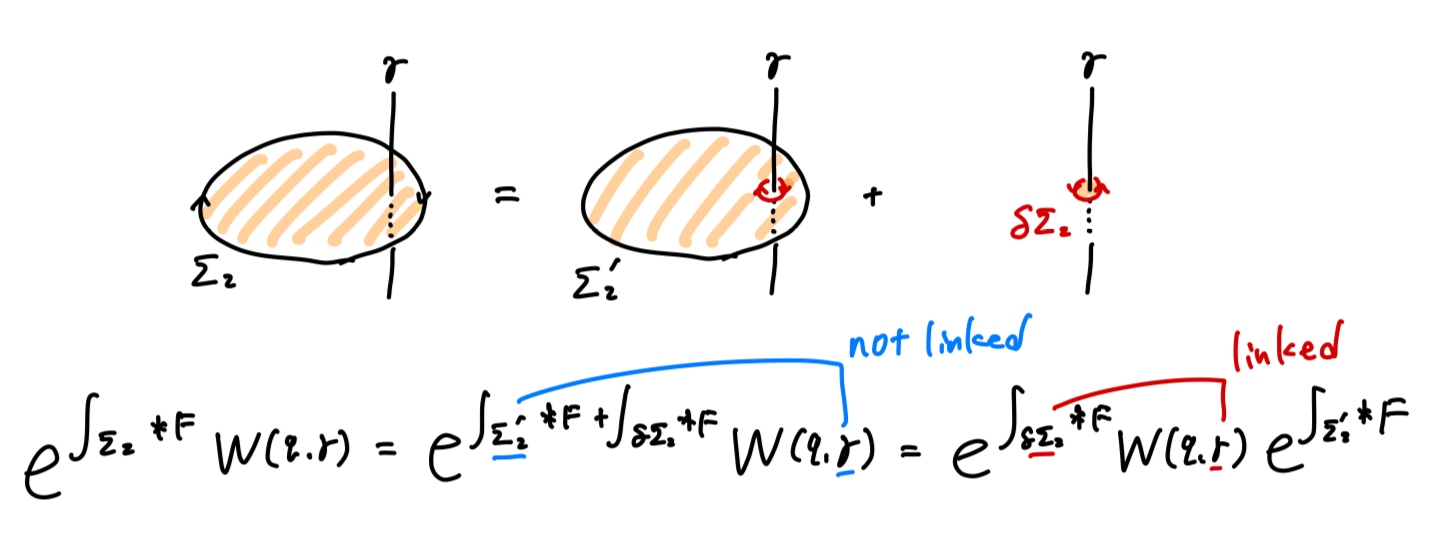
\includegraphics[width=0.8\textwidth]{ActionToWilsonLine.jpg}
    \caption{$\Sigma_2=\Sigma'_2\cup \delta \Sigma_2$, where $\Sigma_2$ is a boundary of infinitesimal $3$-dim mfd which links to $\gamma$. }
    \label{ActionToWlison}
\end{figure}
\noindent
Note that this deformation should be interpreted in path-integral formulation. Thus, we have
\begin{align}
    \lr{\exp\blr{i\frac{\lambda}{g^2}\oint_{\Sigma_2}\star F}W(q, \gamma)}
    =\lr{e^{iq\lambda\mathrm{Link}(\Sigma_2, \gamma)}
    W(q, \gamma)\exp\blr{i\frac{\lambda}{g^2}\oint_{\Sigma'_2}\star F}W(q, \gamma)}, 
\label{WlisonLineCharge}
\end{align}
which is the same as \eqref{ActionWilson}. \\
 By the way, the action of $U^e_\lambda$ on $W(q, \gamma)$ can be seen as the shift of 1-form gauge field $A$ by 
 $A\mapsto A + a$, where $\oint_{\gamma} a =\lambda \mathrm{Link}(\Sigma_2, \gamma)$. 
 In fact, the associate current $\star J^e$ is the conjugate momentum of $A$, generating the shift of $A$. \\
 \\
 We can also consider the "dual" $1$-form symmetry: due to the Bianchi identity, we have $dF=0$ (that is, the pure Maxwell field is flat). 
 By regarding this identity as the conservation of $2$-form current $J^{m}_2 :=\frac{1}{2\pi}\star F$, we can write down the correponding symmetry operator as
 \begin{align}
    U^{m}_\lambda(\Sigma_2) = \exp\blr{i\lambda\oint_{\Sigma_2}\star J^m_2}
    =\exp\blr{i\lambda\oint_{\Sigma_2}\frac{F}{2\pi}}. 
 \label{magnetic1form}
 \end{align}
 This $1$-form symmetry is called \textit{magnetic $1$-form symmetry}. Its charged operator is the so-called \textbf{'t Hooft line}
 \begin{align}
    T_1(m, \gamma) := e^{im\int_{\gamma}\tilde{A}}, 
 \label{tHooft}
 \end{align}
 where $\tilde{A}$ is the dual gauge field defined by $\star F=d\tilde{A}$. 
 The action of the $1$-form magnetic symmetry on a 't Hooft line is completely analogous to the case of electric $1$-form symmetry: 
 \begin{align}
    \lr{U^{m}_\lambda(\Sigma_2)T_1(m, \gamma)}
    =e^{im\lambda\mathrm{Link}(\Sigma_2, \gamma)}\lr{T_1(m, \gamma)U^{m}_\lambda (\Sigma'_2)}. 
 \label{ActionTotHooft}
 \end{align}
\\ \\
It is insightful to consider coupling "background $1$-form $U(1)$ gauge field" to our conserved $2$-form currents, as we have done in the case of ordinary $U(1)$ gauge theory. 
This is done by modifying the action integral
\footnote{詮: 系の力学を記述する「作用積分」と, 演算子の場に対する「作用」を区別するために, 以降は前者を"action integral"と呼ぶことにします. }
\begin{align}
    S=\frac{1}{2g^2}
\label{Gauging1formSym}
\end{align}
\subsection{}
\section{Non-invertible symmetry}
%ここからは, 先に述べた「2つの一般化の方向」の, もう一つに視点を当ててみる. 
%今までの議論において, 対称性演算子には常にその逆元が存在していた. 
%いま, そのような制約を緩めた時にどのような「対称性」が現れるのかを考える. 
%これはもはや通常のgroup-likeな対称性ではなく, 「非可逆対称性」あるいは"non-invertible symmetry"と呼ばれるものになる. \\
 

%非可逆的対称性の持つ代数構造は群をなさないが, それはフュージョン圏と呼ばれる圏の構造を有している. 
%もう少しだけ言うと,非可逆対称性を持つ理論において, そこに現れるsymmetry defect operatorたちの間には"fusion rule"という関係があり, 
%これはdefect同士を"fuse"して別のdefectを生み出すという点で, defectとdefectの間の射であるとみなせる. 
%すると, (simple) defectを対象, defect同士の変換則=fusion ruleを射とした圏を考えることができるが, 
%この圏にはテンソル積および"F-symbol"という自然変換が備わっているという点で, 
%一般の圏よりも代数的に「豊かな構造を持っている」圏(=フュージョン圏)をなすということがわかる. \\
Let us now turn our attention to the other of the “two generalization directions” mentioned earlier. 
In the previous discussions, symmetry operators have always had their inverses. 
Now, let us consider what kind of “symmetry” will appear when such restrictions are relaxed. 
This is no longer the usual group-like symmetry, but is what we call "non-invertible symmetry" or "non-invertible symmetry". \\
\subsubsection{Algebraic Structure of Non-invertible Symmetry: Fusion Category}
The algebraic structure of non-invertible symmetry is not a group, but it in general has a categorical structure called a fusion category. 
To say a little more, in a theory with irreversible symmetries, there is a "fusion rule" relation between symmetry defect operators that appear in the theory. 
This is regarded as a projection between defect and defect, in that defects "fuse" with each other to create another defect. defects in the sense that defects “fuse” with each other to produce another defect. 
Then, we can consider a category with (simple) defects as "objects" and the fusion rule between defects as "morphisms". 
This sphere has a "richer structure" algebraically than the general sphere 
in that it has a tensor product and a natural transformation called "F-symbol". (=fusion sphere) in that this sphere has tensor products and “F-symbol” natural transformations. 
\\
 The fusion category consists of the following structures: 
\begin{itemize}
    \item tensor functor
    \item natural transformation 
\end{itemize}
 But why we should care about such a categorical structure?
  Note that the algebraic structure of non-invertible symmetry cannot be totally arbitrary: 
  there should be some rules or orders. 
  More precisely, we need some "consistency condition" for valid physical systems. 
\subsubsection{Example from lattice}
The (probably) most typical example of field theory with non-invertible symmetry is 
of the critical transverse-field Ising model (TFIM). Its Hamiltonian is given by
\begin{align}
    H = -\sum_{j=1}^{L}(Z_{j-1}Z_j + X_j), 
\end{align}
with periodic boundary condition $X_j = X_{j+L}, Z_j=Z_{j+L}$. 
This model has $\zet_2$ symmetry
\subsubsection{Example from continuous}
\section{What comes next?}
In this section, we will see what comes as following topics after studying gerenalized symmetry in this text. 
I appologize that I do not understand the following topics and cannot explain any details. 
\subsection{Generalized charges}
\subsection{Symmetry TFT}
\begin{thebibliography}{99}
    %\bibitem{Hidaka} \href{}{}
    \bibitem{TDBSH} T. Daniel Brennan, Sungwoo Hong. 
    Introduction to Generalized Global Symmetries in QFT and Particle Physics. \href{https://arxiv.org/abs/2306.00912}{\texttt{arXiv: 2306.00912}}
\end{thebibliography}
\end{document}